% !TeX encoding = UTF-8
% !TeX program = xelatex
% !TeX spellcheck = en_US

%-----------------------------------------------------------------------
% 中国科学: 信息科学 中文模板, 请用 CCT-LaTeX 编译
% http://scis.scichina.com
% 南开大学程明明注释:也可以在Overleaf中使用XeLaTeX直接编译,
% 例如:
%-----------------------------------------------------------------------

\documentclass{SCIS2020cn}
%\usepackage{breakurl}
%\captionsetup[subfloat]{labelformat=simple,captionskip=0pt}


%%%%%%%%%%%%%%%%%%%%%%%%%%%%%%%%%%%%%%%%%%%%%%%%%%%%%%%
%%% 作者附加的定义
%%% 常用环境已经加载好, 不需要重复加载
%%%%%%%%%%%%%%%%%%%%%%%%%%%%%%%%%%%%%%%%%%%%%%%%%%%%%%%


%%%%%%%%%%%%%%%%%%%%%%%%%%%%%%%%%%%%%%%%%%%%%%%%%%%%%%%
%%% 开始
%%%%%%%%%%%%%%%%%%%%%%%%%%%%%%%%%%%%%%%%%%%%%%%%%%%%%%%
\begin{document}

%%%%%%%%%%%%%%%%%%%%%%%%%%%%%%%%%%%%%%%%%%%%%%%%%%%%%%%
%%% 作者不需要修改此处信息
\ArticleType{论文}
%\SpecialTopic{}
%\Luntan{中国科学院学部\quad 科学与技术前沿论坛}
\Year{2020}
\Vol{50}
\No{1}
\BeginPage{1}
\DOI{}
\ReceiveDate{}
\ReviseDate{}
\AcceptDate{}
\OnlineDate{}
%%%%%%%%%%%%%%%%%%%%%%%%%%%%%%%%%%%%%%%%%%%%%%%%%%%%%%%

\title{水环境中抗生素的主要来源和残留分析}{引用的标题}

\entitle{Title}{Title for citation}

\author[1,2]{作者1}{}
\author[2]{作者2}{{abc@xxxx.xxx}}
\author[1]{作者3}{}
\author[3]{作者4}{}

\enauthor[1,2]{Ming XING}{}
\enauthor[2]{Mingming XING}{{abc@xxxx.xxx}}
\enauthor[1]{Ming XING}{}
\enauthor[3]{Ming XING}{}

\address[1]{作者单位, 城市 000000}
\address[2]{作者单位, 城市 000000}
\address[3]{作者单位, 城市 000000}

\enaddress[1]{Affiliation, City {\rm 000000}, Country}
\enaddress[2]{Affiliation, City {\rm 000000}, Country}
\enaddress[3]{Affiliation, City {\rm 000000}, Country}

\Foundation{基金资助}

\AuthorMark{第一作者等}

\AuthorCitation{作者1, 作者2, 作者3, 等}
\enAuthorCitation{Xing M, Xing M M, Xing M, et al}

%\comment{\dag~同等贡献}
%\encomment{\dag~Equal contribution}

\abstract{抗生素在水生环境中的残留引起了人们的广泛关注,因为它可能导致细菌出现耐药性,从而降低抗生素的治疗效果。由于在农业和人类医疗的不合理地使用抗生素,使得这一问题更加严重。此外,由于缺乏适当的污水处理设施会导致抗生素在水生环境中的广泛扩散。本文的目的是全面综述水生环境中抗生素的所有相关来源。除了来自水产养殖和畜禽养殖等常见抗生素来源外,还包括将抗生素大量释放到水环境中的其他活动。研究了与这些来源相关的抗生素种类和环境中残留情况,以说明水生环境中抗生素存在的危害}

\enabstract{An abstract (about 200 words) is a summary of the content of the manuscript. It should briefly describe the research purpose, method, result and conclusion. The extremely professional terms, special signals, figures, tables, chemical structural formula, and equations should be avoided here, and citation of references is not allowed.}

\keywords{关键词1, 关键词2, 关键词3, 关键词4, 关键词5}

\enkeywords{keyword1, keyword2, keyword3, keyword4, keyword5}

\maketitle
\makeentitle

\twocolumn[]
\setcounter{section}{-1}
\section{前言}
抗生素广泛应用于人类和动物疾病的治疗和预防 [1],是治疗人类和动物感染性疾病的有效药物或者疾病预防药物,而且抗生素也被作为生长促进剂在畜牧业中大量应用 [2]。我国是抗生素生产和使用大国。我国被认为是“世界上滥用抗生素问题最严重的国家之一 [3]。据相关研究报道,我国在2013年抗生素总使用量达162万吨,其中48%为人用抗生素,其余为畜牧用抗生素,抗生素人均年消费量为138g左右,而美国仅为13g,是美国的10倍 [4]。
抗生素的生产和使用导致人类和动物死亡率和发病率显著降低。但是抗生素的大量生产和消费也导致了抗生素在环境中随处可见的情况 [5]。在水环境中如湖泊、河流、水库、污水处理厂的进水和出水,地下水甚至已经处理过的饮用水中都发现了抗生素的存在 [6,7] 。抗生素的潜在危害是即使在是低浓度环境下也会使细菌产生耐药性,产生超级细菌 [8,9]。因此,抗生素是被认为是新出现的环境污染物 [6],抗生素的过度使用和滥用是细菌耐药性产生和扩散的关键因素。
水环境中的抗生素来源于各种方面:城市污水(医院和市政污水,包括家庭废水大部分) [10,11] ,农业(水产养殖、畜牧业) [12,13]和制药企业 [14](见图1)。每个来源在不同的国家和地区的贡献程度是不同的。例如,德国的畜禽养殖和水产养殖的贡献很小,而人类医疗是主要来源(Hirsch等人,1999年)。在台湾,与水产养殖和污水处理厂的废水相比,制药企业是抗生素的主要来源(Lin等人,2008年)。
随着我国经济的飞速发展,抗生素的使用已经非常普遍,抗生素在环境中的残留对生态系统和人类健康已经构成了重大威胁,引起人们高度关注。抗生素治理问题已经刻不容缓,但是目前的常规污水处理方法对抗生素的去除率很低(列举几个文献) ,无法有效去除污水中抗生素,从源头阻止抗生素进入水环境中是一种行之有效的方法。
因此,本综述旨在从源头分析抗生素污染物的来源和在环境中的残留情况,阐述抗生素在环境水域的应用情况。为了解抗生素在水环境中的概况,提供更加全面的情况,并为控制抗生素污染的政策提供依据。


%正文开始 \cite{ref,author}.
%%%
%\begin{definition}[定义名,可省略]\label{def1}
%这是一个定义.
%\end{definition}
%%%%
%\newpage

图片如\ref{fig1}所示.
\begin{figure}[ht]
\centering
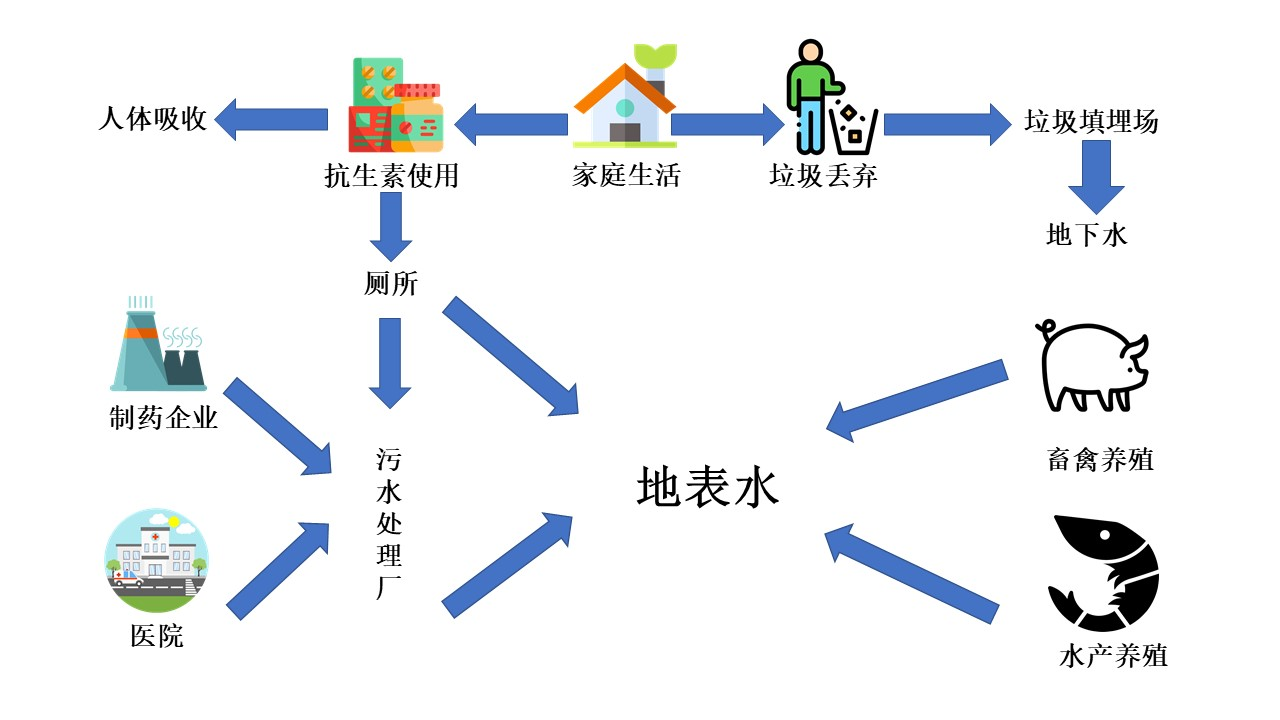
\includegraphics[scale=0.25]{1.jpg}

\cnenfigcaption{抗生素进入水环境的途径}{Caption}
\label{fig1}
\end{figure}

\section{水中抗生素来源}
\subsection{医疗}
\subsubsection{医院中抗生素使用情况}
据2006-2007年度卫生部全国细菌耐药监测结果显示,全国医院抗菌药物年使用率高达74%[15] 。而在美英等发达国家,医院的抗生素使用率仅为22%~25% [16]。在级别较低的医院和中国西部地区,过度使用抗生素的问题严重。估计约有75%的季节性流感患者使用抗生素,住院患者的抗生素处方率为80%,远远高于世界卫生组织建议的最高水平30%[17]。特别地,在外科住院患者的治疗过程中,抗生素药物使用比例更是高达 97%,这导致我国成为全球抗生素滥用最严重的国家之一[18]。医院使用的抗生素药物主要包括:青霉素类 和β-内酰胺酶抑制剂、头孢菌素类、单环内酯类、大环内酯类、喹诺酮类、糖肽多粘素、咪唑衍生物、呋喃衍生物和其它抗生素(包括四环素、氨酚、磺胺类、甲氧苄啶和氨基糖苷类抗菌剂) [19]
直到2011年中国卫生部发起的人体医疗体制改革,中国才开始有效控制抗生素的处方模式 [20]。据报道,接受抗生素处方的住院患者比例在一年内下降了10%,从2011年的68%下降到2012年底的58%。在同一时期,门诊患者的比例也从25%下降了10%~15%。干预后普通医院的住院抗生素总体消费量显着下降 [21]。但根据30多个省份共151医院的抗生素使用数据显示,2011-2014年抗生素的总体使用量有所下降 ,但是广谱抗生素的使用在稳定增加,特别是头孢菌素,占所有抗生素使用量的50% [19]。贵州某医院2013年至2016年度具有抗生素处方占比分别为50.8%、54.2%、49.2%、49.2%, 4年抗生素使用的比例平均为50.9%, 而根据国家卫生部门的相关规定, 门诊处方中抗生素的使用率不得超过20%,其比例远超国家规定 [22]。在佛山某医院2018-2019年所有的处方中,头孢类的使用率最高,为49.00%,青霉素类次之,为22.43%[23]。有研究表明,头孢类抗生素的使用频度与耐药细菌的产生呈正相关,耐药菌产生的主要原因之一为头孢类抗生素的使用 [24]。
造成中国滥用抗生素的因素有很多。首先,许多医生认为广谱抗生素是治疗多种感染最有效的方法,并依赖于经验性治疗 [19]。其次,患者对抗生素不了解,认为这些药物会更有疗效。最关键的是,中国复杂的卫生体系,加上医生开出更多药物的经济激励措施,很可能会影响药物的合理使用[25]。抗生素的大量使用容易造成人体内菌群失调、破坏正常菌群结构、产生大量耐药菌株,使患者的药物使用量越来越大,增加患者的疾病负担。抗生素的抗菌效果大同小异,很多时候医师在开具处方时,药物作用相近,重复用药,导致患抗生素耐药,增加了患者不良反应等。基层医院住院患者抗生素不合理用药现象普遍存在,应该全面加强用药管理,制定目标性的管理制度,禁止抗生素滥用。 [26] 

\subsubsection{医院废水抗生素残留}
我国是抗生素的使用大国,人口众多,加之医生对抗生素滥用的情况严重,这就造成了医院废水中含有大量的抗生素,而且我国医院污水多采用一级强化处理工艺 [27],简易的混凝沉淀并不能有效去除医院污水中残留的抗生素。有研究证实医院废水是自然水体中抗生素的主要来源之一 [28]。
大多数在医院废水中发现的抗生素浓度较高,远远超过城市河流水或城市废水,特别是头孢类、喹诺酮类和四环素类抗生素 [29,30]。在其他医院废水中也报告了类似的结果 [31,32]。这可能归因于它们的大量的医疗消耗[33] 。不同类别医院废水中的抗生素总类也有很大区别,
对海口市3 家医院废水中的抗生素类药物残留研究发现,医院废水中 6 种抗生素的浓度介于 3.546 μg/ L 至 53.356 μg/ L 之间,远远高环境水体抗生素的浓度水平。
6 种抗生素的去除率介于 36.3~100\% [34]。

\subsection{水产养殖}
\subsubsection{水产养殖中抗生素使用情况}
在我国,随着国内水产养殖集约化的不断发展,水产养殖单位面积产量显著增加,在养殖中使用抗生素来治疗或预防感染和促进生长已经成为一种常见做法。抗生素显著的抗菌能力和低副作用使其成为水产养殖上疾病防治的常用药物。常用于水产养殖的抗生素:应用在水产养殖中的抗生素种类主要有喹诺酮类、磺胺类、四环素类、大环内酯类、氨基糖苷类等,其中四环素类抗生素已经在水产养殖业中广泛使用,具有广谱性和低毒性等特点。已有报道的四环素类抗性基因就有40多种在水产养殖业中传播和扩散【8】。

中国在水产养殖上投入了大量资金,是全球最大的养殖鱼类生产国 [35]。为了维持高种群密度的水产养殖,需要大量投入,包括饲料,改良剂,有机肥料以及抗生素等药物(Bosma和Verdegem,2011),来预防多种细菌性疾病(Heuer等,2009)。人们对水产养殖生态系统中抗生素使用的增加已经引起广泛关注(Seyfried等,2010; Xiong等,2015)。根据对中国河流流域抗生素排放和来源的综合评估,2013年,包括鱼类在内的食用动物养殖量为13,700吨,占抗生素总量的80%以上(Zhang等人,2015)。 与智利的鲑鱼养殖相似,药物饲料和直接喷洒是中国抗生素管理的主要方法(Shah等人,2014)。消化或未消化的抗生素将最终出现在水产养殖周围的水环境中(Cabello等,2013)。水中的抗生素负担最终将成为水产养殖生态系统的潜在生态风险,例如抑制水生生态系统生物地球化学功能所依赖的初级生产力(Andrieu等人,2015)。诸如氮吸收,有机物氧化之类的生态系统功能可能会由于初级生产力的丧失而受到阻碍(Celine and Anniet,2015)。但是,最近的研究尚未很好地探索中国水产养殖环境中抗生素使用的特征(Chen等人,2015)。

养殖区使用喹诺酮类抗生素较普遍

郝红珊等对大亚湾、珠海的渔业养殖区进行采样分析,在海水中检出6中抗生素奇霉素(4.68ng/L),氧氟沙星(3.19ng/L),诺氟沙星(2.09ng/L),头孢噻肟钠(1.58ng/L),甲氧苄氨嘧啶(0.54ng/L)和磺胺甲恶唑(0.13ng/L)、沉积物中13中抗生素、生物样(鱼类和贝壳)中18种抗生素。 [36]

在中国,用于水产养殖的抗生素超过30种属于磺胺的抗生素,BACT法AM、Quinolones、大环内酯、CYCYLINES和一些其他抗生素组被允许以有限的量使用(表2)。同时,一些广谱抗生素如氯霉素,大多数氟喹诺酮类和硝基咪唑类被禁止在水产养殖中使用,因为它们对人类健康可能对水产养殖产品的消费产生影响(MARD,2014年)。蚂蚁数越南可用于水产养殖的益生菌远高于其他国家,如美国,那里只有4种抗生素(土霉素、氟苯尼考、磺胺嘧啶和orme)。可用于水产养殖(Chuah等人,2016年)。由于这个行业允许大量使用抗生素,因此很难控制抗生素的使用,并有可能增加使用抗生素的风险。不合理使用和环境污染。


抗生素在水产养殖中的应用因品种和养殖阶段的不同而不同。根据TAI(2004),越南376种水产养殖产品中有138种抗生素制剂。NG占36.7%。每种抗生素产品的数量是不同的。例如,在生产虾幼虫的98种产品中,有39种含有抗生素(39.8%),而海洋鳍鱼14/29(48.3%),淡水鱼41/74(55.4%),池塘养殖鱼31/67(46.3%)。值得注意的是,瑞科等人的一项调查。(2013年)报告100%使用抗生素在Pangasius农场,只有2.9%的虾养殖场使用这类药物。越南的养鱼场使用抗生素的比例大大高于其他国家(泰国的罗非鱼养殖场)。土地:9.7%;中国:16%)。越南的Pangasus农场也使用了更广泛的抗生素,涵盖10种不同种类(青霉素、氨基葡萄糖、头孢菌素、五氯硝基苯、四环素S,Amphenicol,多粘菌素,二氨基比林,利福霉素和磺胺类药物)。最常见的抗生素为恩诺沙星(Quinolone)(69%农民)、氟苯尼考(Amphenicol)(63%)、SulfamoXA(磺胺类药物)与三甲基环(44%)、强力霉素(CYCYLINES)(34%)联合使用。平均每个农场使用3种不同的抗生素产品,10%用于5E6抗生素产品。一些产品中甚至含有不同抗生素的混合物(磺胺二甲氧基肟和奥美普林;磺胺甲恶唑和甲氧苄啶;阿普拉霉素和左氧氟沙星)。喹诺酮类抗生素,特别是氟喹诺酮类抗生素,由于其在水和沉积物中的相对稳定性而成为使用最广泛的合成抗生素(Le和Munekage,2004年)。现已禁止使用ES(MARD,2014年)。喹诺酮类抗生素用于幼虫期(环丙沙星)和幼虫后至成虫期(诺氟沙星、恶丙酸)(Thuy等人,2011年)或所有阶段(恩诺沙星)(Pham等人,2015年)。环素用于土霉素、多西环素、金霉素、四环素等幼虫(Pham等人,2015年)。磺胺类抗生素VAE至成人阶段(磺酰胺、甲氧苄啶);磺胺嘧啶;磺胺二甲氧基(Thuy等人,2011年;Pham等人,2015年)。
Antibiotic residues from aquaculture
在接受虾或养鱼业废水的水体中检测到各种抗生素,这些抗生素是由于它们的共同用途而被发现的。据Giang等人说。(2015年),占地表水的91.6%在湄公河三角洲接受水产养殖废水的样本中含有1种抗生素,55,2%含有3e4抗生素。水产养殖废水中发现的抗生素包括磺胺类、大环内酯类、苏铁线和五氯硝基苯(LE和Munege,2004;Takasu等人,2011;Shimizu等人,2013;Andrieu等人,2015;Giangetal.,2015),详见表S1。由于T在水产养殖中广泛使用氟利昂抗生素,它们在不同浓度水平的多种水生环境中经常被检测到。看到ENROF是合理的氧氟沙星是使用最频繁的抗生素,其浓度最高,可达680 ng L,1在从Pangasius猫鱼场排放到c的污水管道处。肛门(Andrieu等人,2015年),高于虾场废水中氧氟沙星和诺氟沙星(分别为238.6 ng L、1 ng和44.4 ng L、1)(Takasu等人,2011年)。值得注意的是,尽管自2009年以来,水产养殖中禁止使用氟喹诺酮类药物,特别是恩诺-氟沙星(MARD,2014年),但据报道,它们仍被用于鲶鱼养殖(Andrieu等人,2015年;G.Iang等人,2015年)以及养虾业(CHI等人,2017年)。抗生素在水产养殖中的广泛应用污染了水,还污染了沉积物相,因为随着未消耗的饲料颗粒的沉淀,抗生素积累在沉积物中。荧光酮抗生素的掺入进入沉积物可能增加了它们在环境中的持久性,随后延长了它们的不利影响(Le和Munege,2004;Andrieu等人,2015;Giang等人,2015)。恩诺沙星在接收到浓度高达59纳克升的水产养殖废水的运河和河流中随处可见,一条运河的浓度高达1纳克(Giang等人,2015年)。其他喹诺酮类抗生素(NOR,LOM和CIP)在虾场、养鱼场场址、与养猪场和鸭场结合的鱼塘收集的地表水和废水中重新检测到。综合耕作制度可能是经济上有益的,但是因此,从畜牧业到水产养殖都有污染抗生素的风险(Hoa等人,2011年)。虾池地表水中乐果酸和NOR浓度在0.01~2.5mg L,1和fr范围内。约0.06至6.06毫克L1,类似于在周围运河的地表水中测量的水平(Le和Munekage,2004年)。在与养猪场整合的鱼塘中检测到LOM,浓度可达3。5.9纳克L,1(Takasu等人,2011年)。虾场废水中没有检测到CIP和LOM(Takasu等人,2011年)。SMX、SDZ和TRI的检测频率很高(Le和Munekage,2004年;Hoa等人)。,2011年;Giang等人,2015年)。这与磺胺e类产品的普遍使用是一致的。其他磺胺类药物,如stz、smr、smz、sdx等,在对虾样本中均未检出。农场和猪/鱼场(HoAetal.,2011)。虾场水中SMX浓度最大为2.39mg/L1(Le和Munege,2004),比914N的虾场废水高出数倍。GL1(HoA等人,2011;Shimizu等人,2013)。周围运河底层的SMX与池水中的SMX一样高(约5.57mgL1)(LeandMunege,2004)。虾仁中的三浓度FARM水高达2.03 mg L,1毫克,约1.2毫克L,周围运河底水1毫克(Le and Munekage,2004年),废水最高85纳克L,1纳克(Hoa等人,2011年)。检测到SMX和SDZ从孵化厂和Pangasius农场接收废水的运河中的可比浓度(分别为135纳克和108纳克升,1纳克)(Giang等人,2015年)。然而,在鱼塘废水中猪场的SDZ浓度可能比SMX高10倍,分别为6662纳克升、1纳克和625纳克L,1(Hoa等人,2011年)。观察到两种化合物的浓度差异。f SDZ浓度高于SMX 28倍的鱼塘/鸭池(1966 ng L,1和70 ng L,1)(Shimizu等人,2013年)。因此,本文认为SMX主要用于虾池,而SDZ则主要用于虾池。在与鱼塘相结合的养猪场中更为占优势(Hoa等人,2011年)。然而,在另一项研究中,许多虾场的废水样本中没有检测到SMX(Shimizu等人,2013年)。麦克罗里在越南北部的虾场、鱼塘和猪场都检测到了DES,但是,它们的浓度远远低于城市运河中的浓度,而城市运河被认为受到了严重的影响。(Hoa等人,2011年)。红霉素(ERY)是最常见的大环内酯类药物。在t区对虾养殖场和猪鱼综合养殖场的两种废水样本中都发现了这种物质。其浓度分别为0.28 ng L、1 ng和63.9 ng L、1。CLA浓度较低,最高为0.4ng L,猪场为1。在这些样品中未检出SPI、Roxi和Azi(清水eTAL.,2013)。尽管循环抗生素被广泛使用,但它们在高频和高浓度中没有被检测到,这可能是因为它们快速降解并且不易分析。仅在E研究试图测量越南水产养殖中的抗生素组(Shimizu等人,2013年)。OTC是最常见的环素抗生素,也是唯一在猪/f废水中检测到的抗生素。浓度可达36纳克升的ISH农场,1。对虾养殖废水中OTC、TC的浓度分别为18 ng L、1 ng和17 ng L、1 ng。没有在任何样本中检测到dox。林是唯一的林科在越南的研究中正在调查的Samide抗生素。在猪/鱼场中发现的浓度高达416纳克升,1纳克(Shimizu等人,2013年)。

抗生素还会影响水体细菌群落,张云石等研究了磺胺甲吧恶唑对罗非鱼养殖水体细菌群落的影响,发现磺胺甲吧恶唑在中、高浓度剂量下对养殖水体细菌的生物多样性有不同程度的降低影响显著,使得水体菌群向物种丰度降低、优势种明显的趋势发展。(细菌产生耐药性) [37]


徐磊等人在湖州地区养殖水和底泥中分别检测到9种和13种抗生素,平均浓度在0.1ng/L~428.8ng/L和10.0ng/Kg~3681.6ng/Kg之间,其中养殖水中以磺胺类为主,底泥中以四环素类和喹诺酮类为主。 [38]



中国在水产养殖技术方面投入了大量投资,是全世界最大的养殖鱼类生产国(纳勒等人,2000年;渔业局,2014年)。需要大量的输入来维持高电平STOSTOCK密度水产养殖,包括饲料、改性剂、有机肥料和药物,如抗生素(BoSMA和VerdeGem,2011),其有助于防止多种细菌性疾病(Heuer等,(2009年)。人们十分重视水产养殖生态系统中抗生素使用量的增加(Seyfriet al.,2010年;Xong等人,2015年)。根据抗生素的综合评价2013年,中国江河流域包括鱼类在内的食用动物的排放和归宿为13,700吨,占抗生素总量的80%以上(Zhang等人,2015年)


[35]在中国太湖的周边24个鱼塘进行采样检测,所调查的15类抗生素均在水样中检出,检出频率为2~60%。磺胺类药物最为普遍,磺胺甲恶唑、磺胺甲氧胺、氟苯尼考浓度最高。在2 0 0 0ng /L以上,而其它抗生素水平范围从ND(未检出)到551.18 ng /L,


中国在水产养殖技术方面投入了大量投资,是全世界最大的养殖鱼类生产国(纳勒等人,2000年;渔业局,2014年)。需要大量的输入来维持高电平STOSTOCK密度水产养殖,包括饲料、改性剂、有机肥料和药物,如抗生素(BoSMA和VerdeGem,2011),其有助于防止多种细菌性疾病(Heuer等,(2009年)。人们十分重视水产养殖生态系统中抗生素使用量的增加(Seyfriet al.,2010年;Xong等人,2015年)。根据抗生素的综合评价2013年,中国河流流域的排放和命运,包括鱼类在内的食品动物的农业在2013年负责13700吨,占抗生素总量的80%(Zhangetal.,2015)。
与智利的鲑鱼养殖类似,药物饲料和直接喷溅是中国使用抗生素的主要方法(Shah等人,2014年)。消化或未消化抗生素d最后进入周围的水产养殖环境(Cabello等人,2013年)。水中的抗生素负担最终会对水产养殖生态系统造成潜在的生态风险,例如抑制Primar。e初级生产力的丧失(Celine和Anniet,2015年)。然而,最近的研究还没有很好地探索抗生素在中国水产养殖环境中的使用特点(Chen等人)。2015).
\subsubsection{水产养殖中抗生素的残留情况}

	水产品含有大量的抗生素,容易给人们的健康带来威胁[5]。史
    朝斌对某养殖场研究发现。鱼体中检测出含量超过安全残留量的50%以上的的抗生素有脱水红霉素、甲氧咔啶、环丙沙星、诺氟沙星、培氟沙星。体重正常的成人在食用了这些鱼类产品之后,间接摄入大量抗生素,甚至超过了每日允许值。这些鱼类产品未达到安全食用的 标准,有的甚至超过允许残留量的20%,极有可能给人的健康带来一定的风险[6] 。 [39] 
由于它们的共同使用,在从虾或养鱼中接收废水的水体中检测到了各种基团的抗生素。根据Giang等人(2015),91.6%的地表水从水产养殖接收废水的湄公河三角洲采集的样本含有1种抗生素,55,2%含有3E4抗生素。在水产养殖废水中发现的抗生素,包括:磺胺类、大环内酯类、苏铁线和五氯硝基苯(LE和Munege,2004;Takasu等人,2011;Shimizu等人,2013;Andrieu等人,2015;Giangetal.,2015),详见表S1。
由于氟喹诺酮类抗生素在水产养殖中的广泛应用,它们在不同浓度水平的多种水生环境中经常被检测到。看t是合理的..在PangasusCat-FishFarmi的废水管道排放点处,最高浓度(最高达680ngL1)发现最常见的抗生素帽恩诺沙星浓度最高达680ng/L1。Nto运河(Andrieu等人,2015年),在虾场废水中分别高于氧氟沙星和诺氟沙星(238.6纳克L1和44.4纳克L1)(Takasu等人,2011年)。
值得注意的是,尽管自2009年以来,水产养殖中禁止使用氟喹诺酮类药物,特别是恩诺-氟沙星(MARD,2014年),但据报道,它们仍被用于鲶鱼养殖(Andrieu等人,2015年;G.Iang等人,2015)以及虾养殖(Chi等,2017)。和大量使用抗生素在水产养殖中的应用污染水,但也污染沉积物阶段,因为抗生素积累在沉积物中,随着未消耗的饲料颗粒的沉降。氟喹诺酮类抗生素的掺入进入沉积物可能会增加它们在环境中的持久性,并随后延长它们的不利影响(Le和Munekage,2004年;Andrieu等人,2015年;Giang等人,2015年)。恩诺沙星在运河和河流中普遍存在,在Canal(Giang等人,2015)的浓度高达59ngL1的情况下,这些河流和河流都接收到水产养殖废水。其他五氯苯酚抗生素(NOR、LOM和CIP)在虾场、养鱼场、养猪场和养鸭场收集的地表水和废水中检测到废水。集成的农业系统可能在经济上是有益的,但是,因此给水产养殖带来污染抗生素的风险(HoAetal.,2011)。虾池地表水中的氧和浓度均为0.01~2.5mg/L。0.06至6.06毫克升,1,类似于周围运河地表水的水平(Le和Munekage,2004年)。在与猪场合并的鱼塘中检测到洛美浓度高达3。5.9纳克L,1(Takasu等人,2011年)。虾场废水中没有检测到CIP和LOM(Takasu等人,2011年)。
SMX、SDZ和TRI的检测频率很高(Le和Munekage,2004年;Hoa等人,2011年;Giang等人,2015年)。这与磺胺e类产品的普遍使用是一致的。其他STZ、SMR、SMZ、SDX等磺胺类化合物在虾场和猪场/鱼场的任何样本中均未检测到(Hoa等人,2011年)。虾场地表水最大SMX浓度为2.39mg L,1(Le和MuneShe,2004年),比914ngL1的虾场废水高出数倍(HoAetal.,2011;Shimizu等,2013)。周围沟底的SMX和PO中的SMX一样高。ND水(约5.57mgL1)(LE和Munege,2004)。虾场水中的Tri浓度最高为2.03mg/L1,周围管底部水中约1.2mgL1(Le和Munege,2004)。在废水中达到85ngL1(HoAetal.,2011)。在从幼雏和攀西农场(135和108ngL1)接收废水的运河中检测到具有可比浓度的SMX和SDZ,(Giang等人,2015年)。然而,在与猪场结合的鱼塘废水中,SDZ浓度是SMX的10倍,分别为6662 ng L、1和625 ng L、1(Hoa等人)。2011年)。在SDZ浓度大于SMX(1966ngL1和70ngL1)(Shimizu等人,(2013年)。因此,可以得出结论,SMX主要用于虾池,SDZ在与鱼塘结合的养猪场中更占优势(Hoa等人,2011年)。然而,在另一项研究中,SMX没有在许多虾场的废水样本中检测到(Shimizu等人,2013年)。
在越南北部的虾场、鱼塘和养猪场都检测到了大环内酯类化合物,但它们的浓度远远低于城市运河中的浓度,人们认为这是严重的I型。受到人类活动的影响(Hoa等人,2011年)。红霉素(ERY)是最常见的大环内酯类药物。在对虾养殖场和猪/鱼综合养殖场的两种废水样本中都发现了这一现象。浓度分别为0.28ng/l和最高63.9ng/l。CLA浓度较低,在猪/鱼场最大0.4ngL1。在这些样品中未检测到SPI、ROXI和AZI(SHimizu等人,2013年)。
尽管循环抗生素被广泛使用,但它们在高频和高浓度中没有被检测到,这可能是因为它们快速降解并且不易分析。只有一项研究有试图在越南水产养殖中测量该抗生素组(Shimizu等,2013)。OTC是最常见的CyclinE抗生素,是猪/鱼场废水中唯一检出的一种抗生素。浓度可达36纳克升,1。对虾养殖废水中OTC、TC的浓度分别为18 ng L、1 ng和17 ng L、1 ng。没有在任何样本中检测到dox。林是目前调查中唯一的林可酰胺类抗生素。越南的IES。在猪/鱼场中发现的浓度高达416纳克升,1纳克(Shimizu等人,2013年)。




\subsection{畜禽养殖}
\subsubsection{畜禽养殖常用抗生素}
抗生素耐药性已成为全球健康、粮食安全和发展的主要威胁,尤其是在中低收入国家,如中国。Heddini等人,2009年; 肖等人,2011年; Zhang等人,2006年)。与许多国家一样,中国使用的抗生素中约有一半是牲畜使用的,包括用作生长促进剂以及预防和治疗疾病的用途。Zhang等人,2015年)。2010年,中国是牲畜使用抗生素的最大生产国和消费国,预计到2030年,由于人口增长和对肉类蛋白质需求的增加,畜牧业使用抗生素的数量将增加三分之二。van Boeckel等人,2015年)。经合组织最近的一份报告指出,中国在猪和肉鸡生产中使用抗生素的数量是国际平均水平的五倍,这是由于广泛使用抗生素促进生长,违反政府的抗菌素使用政策,以及由于缺乏使用抗菌药物的知识和技能而滥用抗生素(吴,2019).
\subsubsection{}
在动物养殖中长期使用抗生素类饲料添加剂以及亚剂量使用兽药, 再加上抗生素具有 选择性高、吸收率低的特点,使大量抗生素随粪便和尿液排出 [18]。 国彬等[12]对广州市 18 个规模化养殖场周边土壤进行调查, 其中磺胺二甲嘧啶的浓度较高,平均浓度为 1.75 μg/kg [18]。 Wei 等[11]检测了江苏省 27 家规模化养殖场废水及周边地表水中抗生素的浓度水平,10 种抗生素被检出,养殖废水中磺胺甲嘧啶的浓度最高,可达 211 μg/L,地表水中土霉素的 浓度最高可达 6.83 μg/L [18]





\subsection{制药企业}
\subsubsection{制药废水中抗生素残留}
Kim 等人发现污水厂出水中克拉霉素,立定痛等药物含量大于500ng/L [40]。在江苏省某制药厂污水中检测出十种抗生素,浓度在 1.3ug/L~183.9ug/L 之间不等 [41]。
\subsubsection{}



\subsection{生活污水}
\subsection{日常生活抗生素}
\subsection{生活污水抗生素残留}













%%%%%%%%%%%%%%%%%%%%%%%%%%%%%%%%%%%%%%%%%%%%%%%%%%%%%%%%
表格如表\ref{tab1}所示.
表格如表\ref{tab1}所示.
\begin{table}[!t]
\cnentablecaption{表题}{Caption}
\label{tab1}
\footnotesize
\tabcolsep 49pt %space between two columns. 用于调整列间距
\begin{tabular*}{\textwidth}{cccc}
\toprule
  Title a & Title b & Title c & Title d \\\hline
  Aaa & Bbb & Ccc & Ddd\\
  Aaa & Bbb & Ccc & Ddd\\
  Aaa & Bbb & Ccc & Ddd\\
\bottomrule
\end{tabular*}
\end{table}

\subsubsection{三级标题}
算法如算法\ref{alg1}所示.
\begin{algorithm}
%\floatname{algorithm}{Algorithm}%更改算法前缀名称
\renewcommand{\algorithmicrequire}{\textbf{输入:}}% 更改输入名称
\renewcommand{\algorithmicensure}{\textbf{主迭代:}}% 更改输出名称
\newcommand{\LASTCON}{\item[\algorithmiclastcon]}
\newcommand{\algorithmiclastcon}{\textbf{输出:}}% 更改输出名称
\footnotesize
\caption{算法标题}
\label{alg1}
\begin{algorithmic}[1]
    \REQUIRE $n \geq 0 \vee x \neq 0$;
    \ENSURE $y = x^n$;
    \STATE $y \Leftarrow 1$;
    \IF{$n < 0$}
        \STATE $X \Leftarrow 1 / x$;
        \STATE $N \Leftarrow -n$;
    \ELSE
        \STATE $X \Leftarrow x$;
        \STATE $N \Leftarrow n$;
    \ENDIF
    \WHILE{$N \neq 0$}
        \IF{$N$ is even}
            \STATE $X \Leftarrow X \times X$;
            \STATE $N \Leftarrow N / 2$;
        \ELSE[$N$ is odd]
            \STATE $y \Leftarrow y \times X$;
            \STATE $N \Leftarrow N - 1$;
        \ENDIF
    \ENDWHILE
    \LASTCON
\end{algorithmic}
\end{algorithm}

%%%%%%%%%%%%%%%%%%%%%%%%%%%%%%%%%%%%%%%%%%%%%%%%%%%%%%%
%%% 致谢
%%% 非必选
%%%%%%%%%%%%%%%%%%%%%%%%%%%%%%%%%%%%%%%%%%%%%%%%%%%%%%%
%\Acknowledgements{致谢.}

%%%%%%%%%%%%%%%%%%%%%%%%%%%%%%%%%%%%%%%%%%%%%%%%%%%%%%%
%%% 补充材料说明
%%% 非必选
%%%%%%%%%%%%%%%%%%%%%%%%%%%%%%%%%%%%%%%%%%%%%%%%%%%%%%%
%\Supplements{补充材料.}

%%%%%%%%%%%%%%%%%%%%%%%%%%%%%%%%%%%%%%%%%%%%%%%%%%%%%%%
%%% 参考文献, {}为引用的标签, 数字/字母均可
%%% 文中上标引用: \upcite{1,2}
%%% 文中正常引用: \cite{1,2}
%%%%%%%%%%%%%%%%%%%%%%%%%%%%%%%%%%%%%%%%%%%%%%%%%%%%%%%
\begin{thebibliography}{99}

\bibitem{ref} Author A, Author B, Author C. Reference title. Journal, Year, Vol: Number or pages

\bibitem{author} 张三, 李四, Author C, et al. Reference title. In: Proceedings of Conference, Place, Year. Number or pages

\end{thebibliography}

%%%%%%%%%%%%%%%%%%%%%%%%%%%%%%%%%%%%%%%%%%%%%%%%%%%%%%%
%%% 附录章节, 自动从A编号, 以\section开始一节
%%% 非必选
%%%%%%%%%%%%%%%%%%%%%%%%%%%%%%%%%%%%%%%%%%%%%%%%%%%%%%%
%\begin{appendix}
%\section{附录}
%附录从这里开始.
%\begin{figure}[H]
%\centering
%%\includegraphics{fig1.eps}
%\cnenfigcaption{附录里的图}{Caption}
%\label{fig1}
%\end{figure}
%\end{appendix}


%%%%%%%%%%%%%%%%%%%%%%%%%%%%%%%%%%%%%%%%%%%%%%%%%%%%%%%
%%% 自动生成英文标题部分
%%%%%%%%%%%%%%%%%%%%%%%%%%%%%%%%%%%%%%%%%%%%%%%%%%%%%%%


%%%%%%%%%%%%%%%%%%%%%%%%%%%%%%%%%%%%%%%%%%%%%%%%%%%%%%%
%%% 主要作者英文简介, 数量不超过4个
%%% \authorcv[zp1.eps]{Ming XING}{was born in ...}
%%% [照片文件名]请提供清晰的一寸浅色背景照片, 宽高比为 25:35
%%% {姓名}与英文标题处一致
%%%%%%%%%%%%%%%%%%%%%%%%%%%%%%%%%%%%%%%%%%%%%%%%%%%%%%%


%\vspace*{6mm} % 调整照片行间距





%%%%%%%%%%%%%%%%%%%%%%%%%%%%%%%%%%%%%%%%%%%%%%%%%%%%%%%
%%% 补充材料, 以附件形式作网络在线, 不出现在印刷版中
%%% 不做加工和排版, 仅用于获得图片和表格编号
%%% 自动从I编号, 以\section开始一节
%%% 可以没有\section
%%%%%%%%%%%%%%%%%%%%%%%%%%%%%%%%%%%%%%%%%%%%%%%%%%%%%%%
%\begin{supplement}
%\section{supplement1}
%自动从I编号, 以section开始一节.
%\begin{figure}[H]
%\centering
%\includegraphics{fig1.eps}
%\cnenfigcaption{补充材料里的图}{Caption}
%\label{fig1}
%\end{figure}
%\end{supplement}

\end{document}


%%%%%%%%%%%%%%%%%%%%%%%%%%%%%%%%%%%%%%%%%%%%%%%%%%%%%%%
%%% 本模板使用的latex排版示例
%%%%%%%%%%%%%%%%%%%%%%%%%%%%%%%%%%%%%%%%%%%%%%%%%%%%%%%

%%% 章节
\section{}
\subsection{}
\subsubsection{}


%%% 普通列表
\begin{itemize}
\item Aaa aaa.
\item Bbb bbb.
\item Ccc ccc.
\end{itemize}

%%% 自由编号列表
\begin{itemize}
\itemindent 4em
\item[(1)] Aaa aaa.
\item[(2)] Bbb bbb.
\item[(3)] Ccc ccc.
\end{itemize}

%%% 定义、定理、引理、推论等, 可用下列标签
%%% definition 定义
%%% theorem 定理
%%% lemma 引理
%%% corollary 推论
%%% axiom 公理
%%% propsition 命题
%%% example 例
%%% exercise 习题
%%% solution 解名
%%% notation 注
%%% assumption 假设
%%% remark 注释
%%% property 性质
%%% []中的名称可以省略, \label{引用名}可在正文中引用
\begin{definition}[定义名]\label{def1}
定义内容.
\end{definition}



%%% 单图
%%% 可在文中使用图\ref{fig1}引用图编号
\begin{figure}[!t]
\centering
\includegraphics{fig1.eps}
\cnenfigcaption{中文图题}{Caption}
\label{fig1}
\end{figure}

%%% 并排图
%%% 可在文中使用图\ref{fig1}、图\ref{fig2}引用图编号
\begin{figure}[!t]
\centering
\begin{minipage}[c]{0.48\textwidth}
\centering
\includegraphics{fig1.eps}
\end{minipage}
\hspace{0.02\textwidth}
\begin{minipage}[c]{0.48\textwidth}
\centering
\includegraphics{fig2.eps}
\end{minipage}\\[3mm]
\begin{minipage}[t]{0.48\textwidth}
\centering
\cnenfigcaption{中文图题1}{Caption1}
\label{fig1}
\end{minipage}
\hspace{0.02\textwidth}
\begin{minipage}[t]{0.48\textwidth}
\centering
\cnenfigcaption{中文图题2}{Caption2}
\label{fig2}
\end{minipage}
\end{figure}

%%% 并排子图
%%% 需要英文分图题 (a)...; (b)...
\begin{figure}[!t]
\centering
\begin{minipage}[c]{0.48\textwidth}
\centering
\includegraphics{subfig1.eps}
\end{minipage}
\hspace{0.02\textwidth}
\begin{minipage}[c]{0.48\textwidth}
\centering
\includegraphics{subfig2.eps}
\end{minipage}
\cnenfigcaption{中文图题}{Caption}
\label{fig1}
\end{figure}

%%% 算法
%%% 可在文中使用 算法\ref{alg1} 引用算法编号
\begin{algorithm}
%\floatname{algorithm}{Algorithm}%更改算法前缀名称
%\renewcommand{\algorithmicrequire}{\textbf{Input:}}% 更改输入名称
%\renewcommand{\algorithmicensure}{\textbf{Output:}}% 更改输出名称
\footnotesize
\caption{算法标题}
\label{alg1}
\begin{algorithmic}[1]
    \REQUIRE $n \geq 0 \vee x \neq 0$;
    \ENSURE $y = x^n$;
    \STATE $y \Leftarrow 1$;
    \IF{$n < 0$}
        \STATE $X \Leftarrow 1 / x$;
        \STATE $N \Leftarrow -n$;
    \ELSE
        \STATE $X \Leftarrow x$;
        \STATE $N \Leftarrow n$;
    \ENDIF
    \WHILE{$N \neq 0$}
        \IF{$N$ is even}
            \STATE $X \Leftarrow X \times X$;
            \STATE $N \Leftarrow N / 2$;
        \ELSE[$N$ is odd]
            \STATE $y \Leftarrow y \times X$;
            \STATE $N \Leftarrow N - 1$;
        \ENDIF
    \ENDWHILE
\end{algorithmic}
\end{algorithm}

%%% 简单表格
%%% 可在文中使用 表\ref{tab1} 引用表编号
\begin{table}[!t]
\cnentablecaption{表题}{Caption}
\label{tab1}
\footnotesize
\tabcolsep 49pt %space between two columns. 用于调整列间距
\begin{tabular*}{\textwidth}{cccc}
\toprule
  Title a & Title b & Title c & Title d \\\hline
  Aaa & Bbb & Ccc & Ddd\\
  Aaa & Bbb & Ccc & Ddd\\
  Aaa & Bbb & Ccc & Ddd\\
\bottomrule
\end{tabular*}
\end{table}

%%% 换行表格
\begin{table}[!t]
\cnentablecaption{表题}{Caption}
\label{tab1}
\footnotesize
\def\tabblank{\hspace*{10mm}} %blank leaving of both side of the table. 左右两边的留白
\begin{tabularx}{\textwidth} %using p{?mm} to define the width of a column. 用p{?mm}控制列宽
{@{\tabblank}@{\extracolsep{\fill}}cccp{100mm}@{\tabblank}}
\toprule
  Title a & Title b & Title c & Title d \\\hline
  Aaa & Bbb & Ccc & Ddd ddd ddd ddd.

  Ddd ddd ddd ddd ddd ddd ddd ddd ddd ddd ddd ddd ddd ddd ddd ddd ddd ddd ddd ddd ddd ddd ddd ddd ddd ddd ddd ddd ddd ddd ddd.\\
  Aaa & Bbb & Ccc & Ddd ddd ddd ddd.\\
  Aaa & Bbb & Ccc & Ddd ddd ddd ddd.\\
\bottomrule
\end{tabularx}
\end{table}

%%% 单行公式
%%% 可在文中使用 (\ref{eq1})式 引用公式编号
%%% 如果是句子开头, 使用 公式(\ref{eq1}) 引用
\begin{equation}
A(d,f)=d^{l}a^{d}(f),
\label{eq1}
\end{equation}

%%% 不编号的单行公式
\begin{equation}
\nonumber
A(d,f)=d^{l}a^{d}(f),
\end{equation}

%%% 公式组
\begin{eqnarray}
\nonumber
&X=[x_{11},x_{12},\ldots,x_{ij},\ldots ,x_{n-1,n}]^{\rm T},\\
\nonumber
&\varepsilon=[e_{11},e_{12},\ldots ,e_{ij},\ldots ,e_{n-1,n}],\\
\nonumber
&T=[t_{11},t_{12},\ldots ,t_{ij},\ldots ,t_{n-1,n}].
\end{eqnarray}

%%% 条件公式
\begin{eqnarray}
\sum_{j=1}^{n}x_{ij}-\sum_{k=1}^{n}x_{ki}=
\left\{
\begin{aligned}
1,&\quad i=1,\\
0,&\quad i=2,\ldots ,n-1,\\
-1,&\quad i=n.
\end{aligned}
\right.
\label{eq1}
\end{eqnarray}

%%% 其他格式
\footnote{Comments.} %footnote. 脚注
\raisebox{-1pt}[0mm][0mm]{xxxx} %put xxxx upper or lower. 控制xxxx的垂直位置

%%% 图说撑满
\Caption\protect\linebreak \leftline{Caption}
